\begin{document}
%=================================================================
%                           Start Document
%=================================================================
\section{Implementation}
\lhead{Implementation} % section header
\setstretch{1.6}
\lhead{Implementation - Software Refactoring}
\subsection{Software Refactoring}
As mentioned introduction wise this project builds upon the work and code base originally developed for the LegoPress \cite{olivier_legopress_2014} in C++ using Qt and further developed by a previous student. However the code quality had become poor with thousands of lines of code and multiple functionalities implemented in a singular file and class. Therefore before continuing on with the project a full refactoring of the code was necessary. The goal being to save time in the long run by creating modular, robust, readable code that could later be further developed for use in clinical trials.

\subsubsection{Documentation}
\begin{figure} [H]
	\centering
	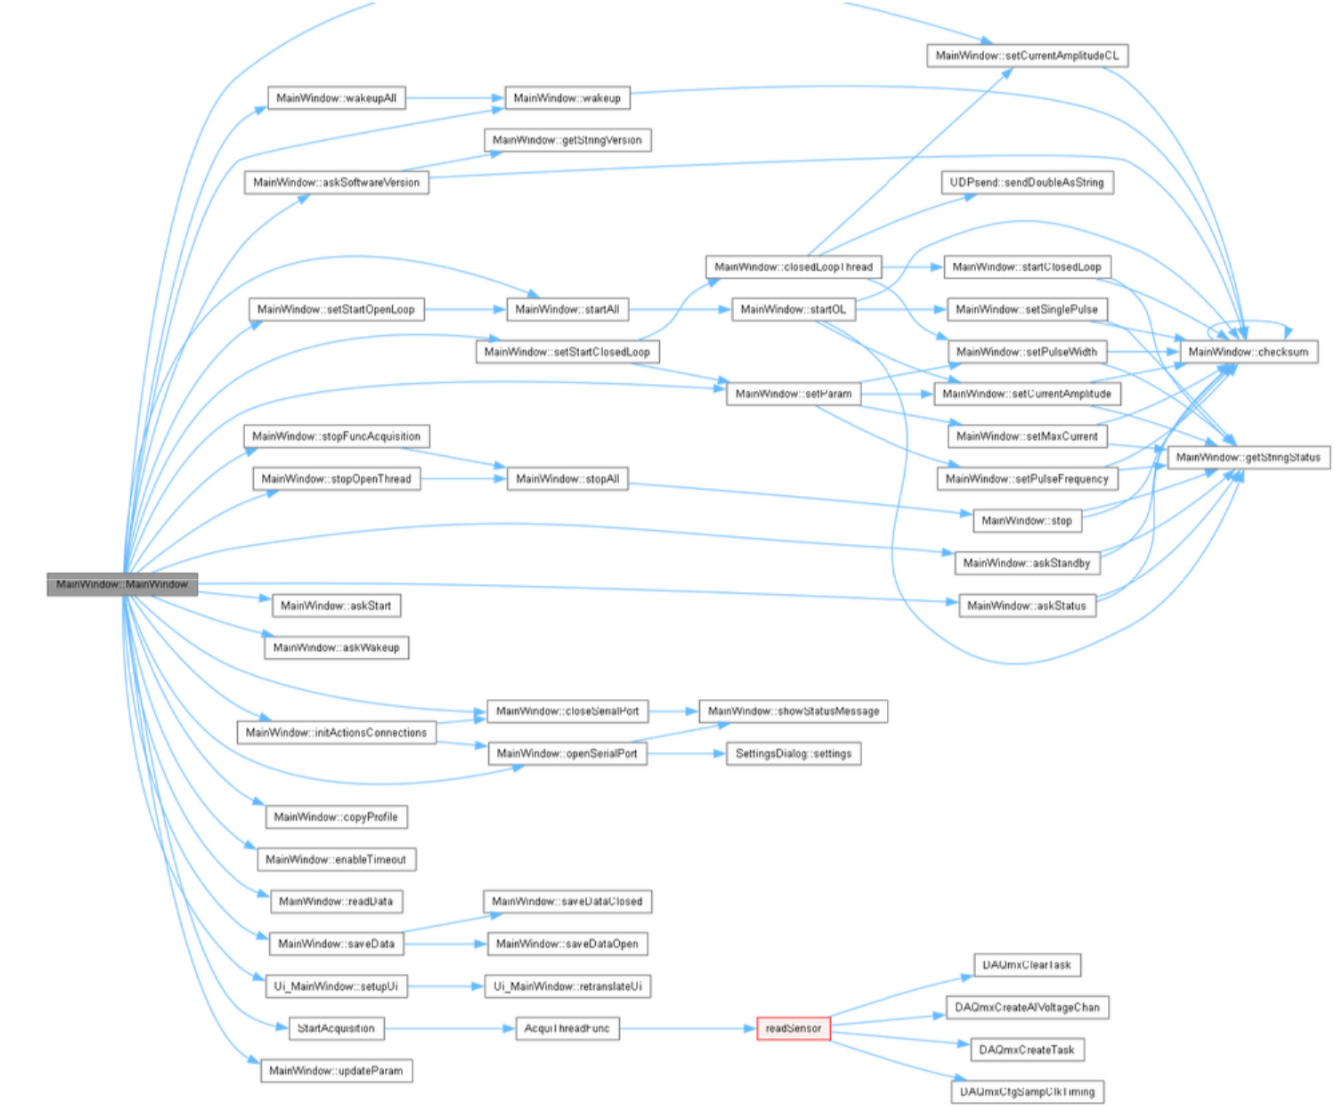
\includegraphics[width=0.9\linewidth]{images/oldDoxy.png}
	\caption{Doxygen generated callgraph for the original mainWindow function before refactoring}
	\label{fig:oldDoxy}
\end{figure}

To gain an understanding of the code and its functionality it was first documented. Specifically it was edited to be compatible with DoxyGen generation of documentation. DoxyGen is a documentation generation tool that automatically creates software documentation in HTML or LateX from annotated source code \todo{source}. This includes graphical representations of callgraphs, such as the one in figure \ref{fig:oldDoxy}, and hierarchies. These are especially helpful when trying to understand the structure and functionality of an unfamiliar code base for the purpose of refactoring and modularization.  \todo{why choose doxygen?}


\subsubsection{Modularization}

In order to improve the code quality modularization and removal of irrelevant functionality was necessary. The code was refactored and divided into classes based on the code quality principles laid out in Code Complete by Steve McConnel \cite{steve_mcconnell_code_nodate}. This includes having clearly defined, minimal interfaces. This is accomplished by using the signal slot mechanism inbuilt into QT, which allows for communication between objects in an event-driven, decoupled manner. Another core concept followed during the modularization process is organizing modules hierarchically, where higher-level modules depend on lower-level modules but not the reverse, thereby avoiding circular dependencies. 

\begin{figure} [h]
    \centering
    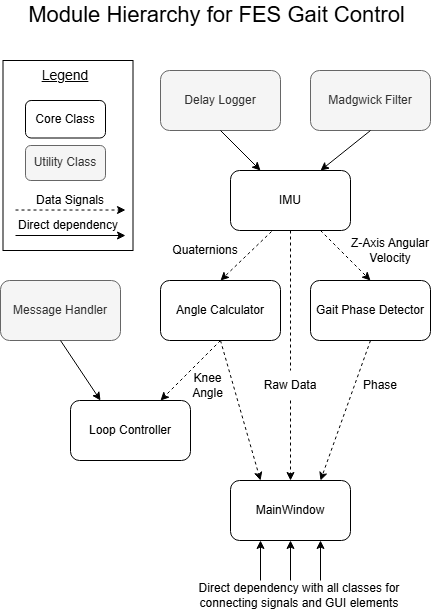
\includegraphics[width=0.6\linewidth]{images/gaitcontrol.png}
    \caption{Module hierarchy after refactoring}
    \label{fig:modulehier}
\end{figure}

A visualization of the hierarchy after refactoring can be seen in figure \ref{fig:modulehier} and description of each class are in table \ref{tab:class-overview}. Previously, all loop controller, IMU functionality, serial communication and bit handling was all done in the mainwindow class. There was also legacy code from the LegopPess, completely irrelevant to this project still in the \texttt{MainWindow} class which was removed. Since this project involved the changing out of the previously utilized wired IMUs with new wireless IMUs, all the code relating to IMU functionality was also removed. The remaining functional code was moved to appropriate classes. These classes are: \texttt{MessageHandler}, \texttt{LoopController} and \textttt{MainWindow}. Additional classes were also added for the new functionality implemented during the project. The final architecture has a high cohesion and low coupling resulting in readable, scalable and testable code that can be effectively reused and further developed upon.




\lhead{Implementation - Functional Electrical Stimulation Setup}
\subsection{Functional Electrical Stimulation Setup}

\subsubsection{Hardware}
The hardware used for the functional electrical stimulation was the StimWave developed at the REHassist lab. It consists of 10 channels where each channel is controlled via an RS-232 line in a master/slave manner. Each electrostimulation channel (slave) has its own address and every command from the FES Gait Control software (master), is dedicated to only one channel. Such that each channel can be used to apply FES to one muscle stimulation site. There is a protocol that describes what each 3 byte command encodes. Using this encoding, the pulse frequency, pulse width, and current amplitude may be adjusted. Along with other commands such as start, stop and status commands. 

\begin{figure} [h]
    \centering
    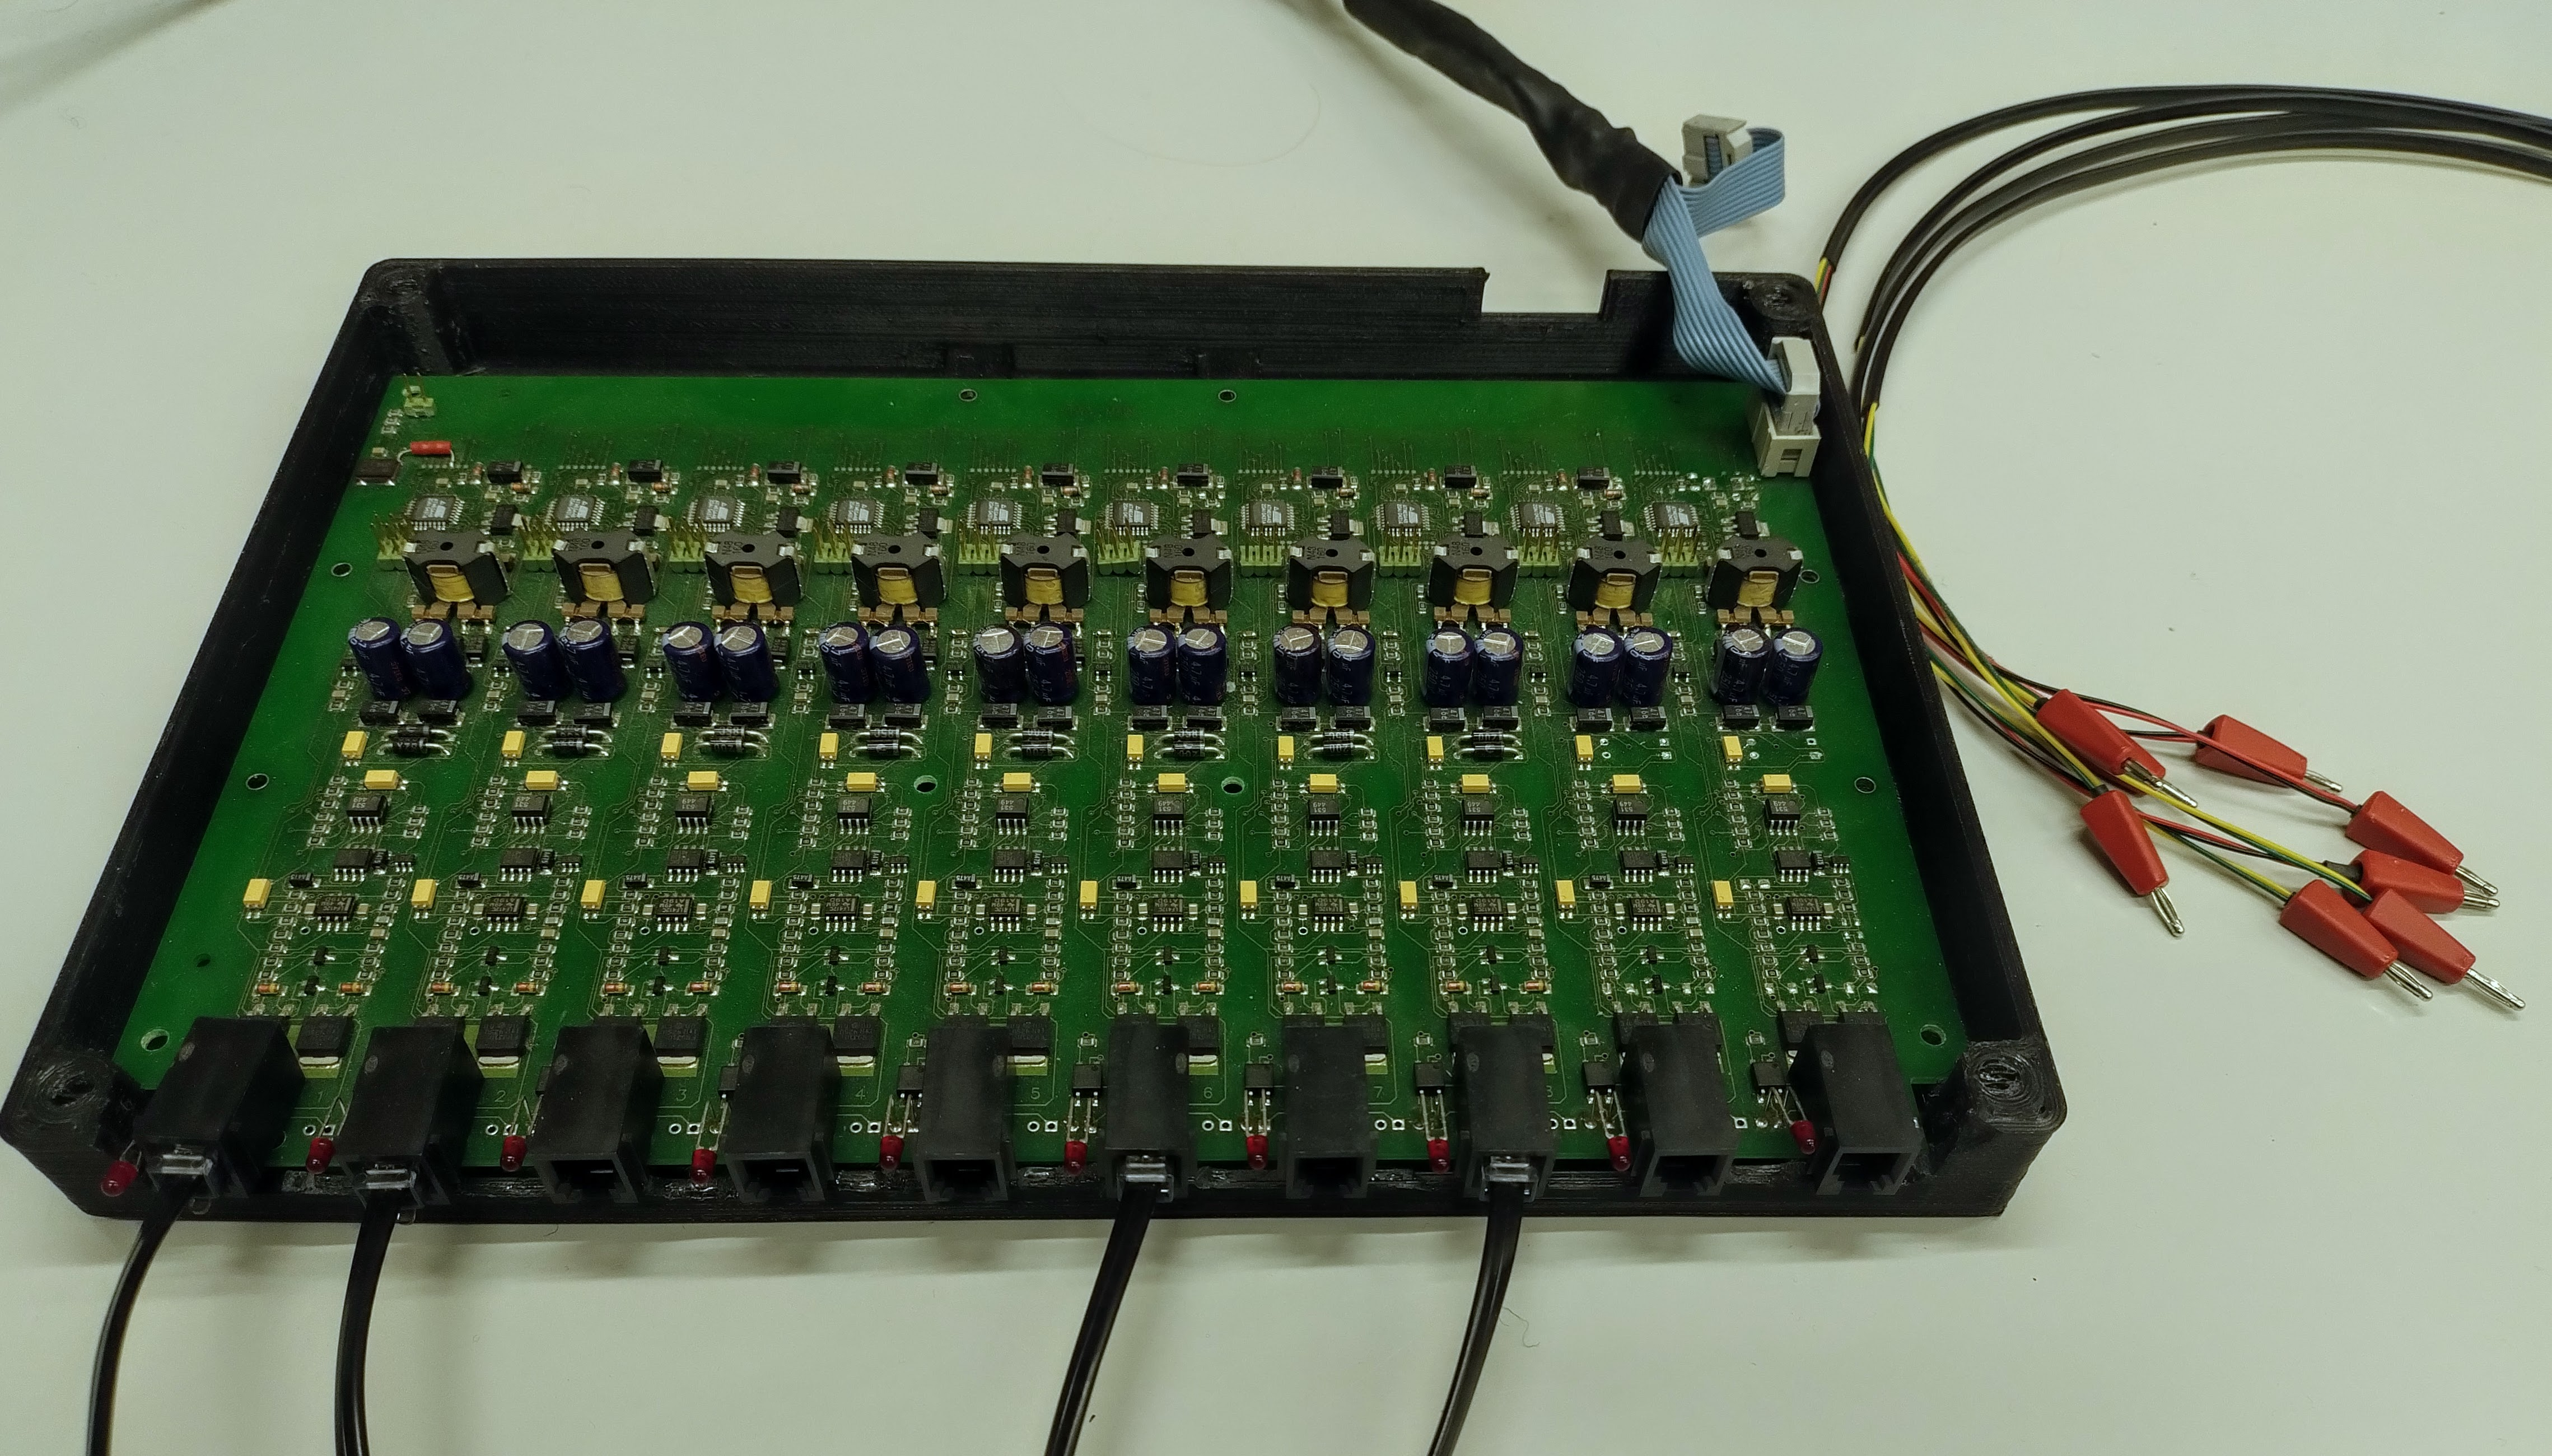
\includegraphics[width=0.8\linewidth]{images/stimwave.jpg}
    \caption{StimWave hardware utilized for FES}
    \label{fig:stimwave}
\end{figure}

However the selection code for the pulse width and frequency had been changed since the implementation used in the original code base. The translation of pulsewidth and frequency in the code therefore needed to be adjusted to the correct 7 bit selection code thereby creating the correct 3 byte commands in the \texttt{MessageHandler} class. The functionality of these changes along with the overall functionality of setting the stimulation parameters was verified using an oscilloscope before moving on to testing FES on subjects. 


\subsubsection{Stimulation waveform}
Stimulus waveforms are generally monophasic or biphasic as seen in figure \ref{fig:twowave}. Monophasic waveforms consist of a single phase of electrical current delivered in one polarity, while Biphasic waveforms consist of a cathodic phase followed by an anodic phase. This mitigates the buildup of charge at the electrode-tissue interface by ensuring that the net charge delivered over time is zero, effectively reducing the risk of tissue damage as compared to monophasic waveforms \cite{peckham_functional_2005}. The biphasic rectangular stimulation is the most commonly used, as it offers the best force-amplitude ratio \cite{lynch_functional_2008}. The balanced biphasic rectangular waveform was therefore chosen for the stimulation protocol used in this project.
 \begin{figure} [H]
     \centering
     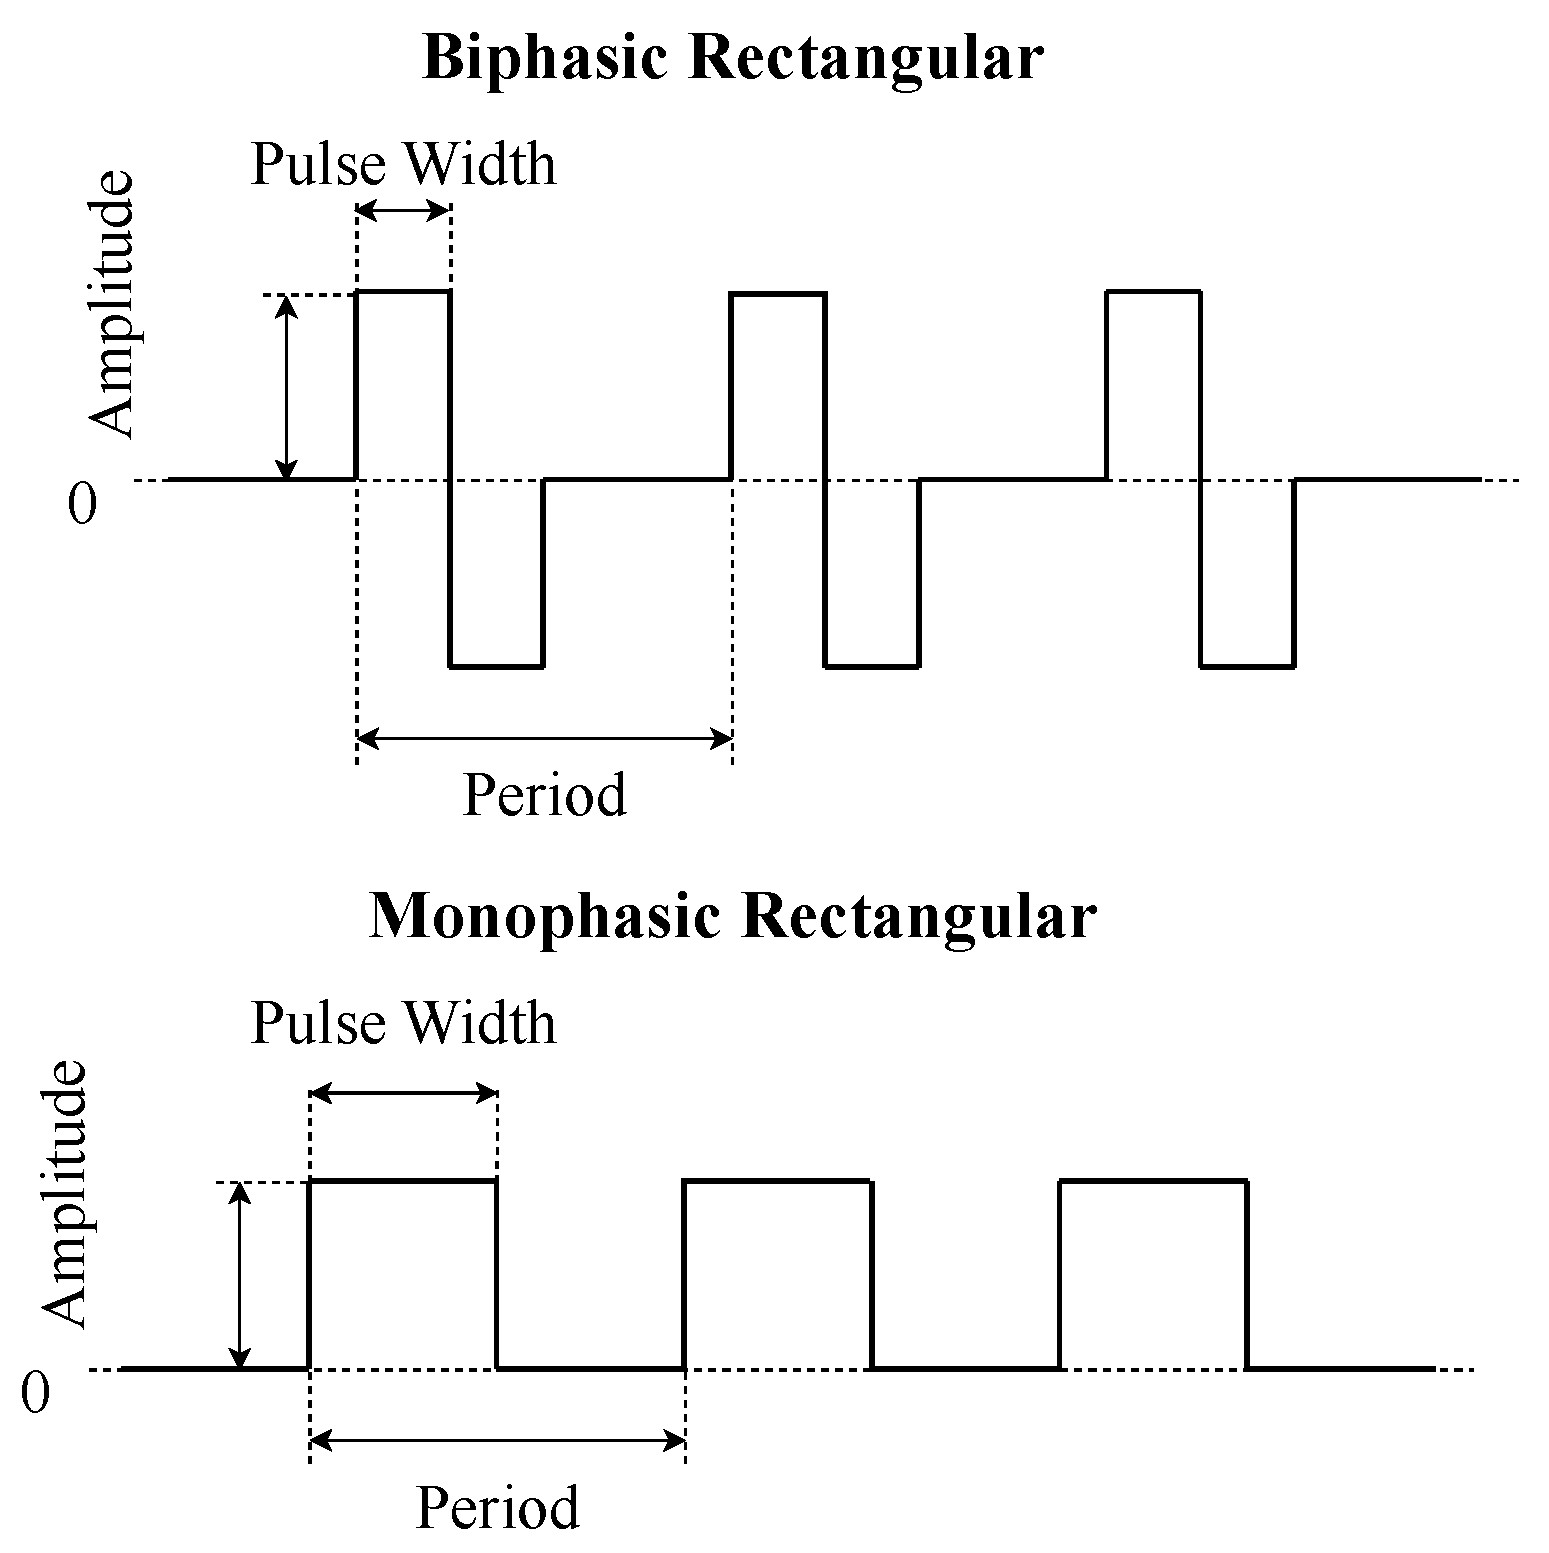
\includegraphics[width=0.6\linewidth]{images/twowaveform.jpg}
     \caption{Monophasic and Biphasic stimulation waveforms}
     \label{fig:twowave}
 \end{figure}
 

\subsubsection{Stimulation frequency}
The stimulation frequency affects the strength of the contraction and its quality. A higher frequency will lead the force produced by each subsequent pulse to be added such that the mean force of the contraction is greater than that produced by a single twitch. Further increase in frequency results in sustained contraction which produces a smooth movement instead of individual twitches. The minimum frequency required to induce fairly consistent contraction is between 16 and 20 Hz \cite{marquez-chin_functional_2020}. A smoother contraction is also more comfortable for the patient \todo{source}. However one should not use a higher frequency than necessary since fatigue accumulated in a muscle is related to the number of pulses received \cite{bigland-ritchie_muscle_2000}. Readers unfamiliar with muscle fatigue are referred to \todo{referral}.

\begin{figure} [H]
    \centering
    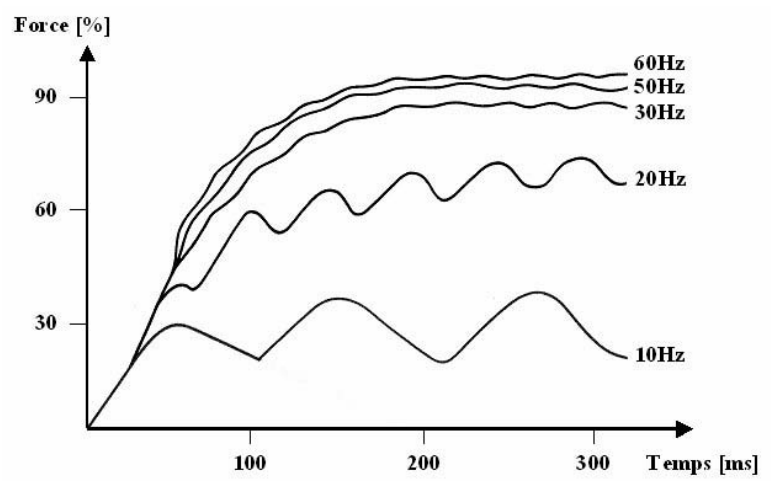
\includegraphics[width=0.7\linewidth]{images/stimfreq.png}
    \caption{Effect of stimulation frequency on force generation \cite{metrailler_systeme_2005}}
    \label{fig:stimfreq}
\end{figure}

When choosing the stimulation frequency the aim was therefore to choose the lowest frequency that produced sustained contractions. In a clinical environment, the typical range of frequencies is around 20-50Hz \todo{source}, and during literature review it was noted that the majority of teams using FES on gait are using a stimulation frequency around 40Hz \cite{aout_effects_2023}. Therefore the same 40Hz stimulation frequency was chosen for this project.



\subsubsection{Stimulation intensity }
The stimulation intensity is determined by the pulse duration as well as the pulse amplitude. To vary the intensity one of the parameters is therefore often kept constant while the other is tuned. 

 \todo{explain better why modulating w amplitude?} 
The pulse duration (pulse width) is the timespan of the stimulation pulse. Higher pulse widths result in more pronounced contraction and enable deeper tissue penetration of the stimulation. Most studies attempting FES for gait employ pulse widths spanning from 200 to 400 \micro s. The majority keep the pulse duration fixed at 300 \micro s and only vary the amplitude in order to set the stimulation intensity.\cite{aout_effects_2023}

The amplitude of the stimulation determines which muscles are contracted and the strength of the contraction \cite{marquez-chin_functional_2020}. Larger amplitudes recruit a larger proportion of the muscle fibers, including those located deeper. 

There are several clinically important values for the amplitude that can be identified. The first is the motor threshold, which is the minimum intensity  that results in a visible muscle contraction, but not necessarily a movement \cite{marquez-chin_functional_2020}. The second is the Maximum tolerable intensity, which is the maximum amplitude that the person can sustain without pain. Finally there is the operational stimulation amplitude, which is the amplitude that produces the intended functional movement needed for the gait cycle. 

These thresholds are highly variable and dependent on both muscle and subject, therefore they are determined here experimentally by slowly ramping up the amplitude for one muscle at a time. Noting when a motor threshold is reached, when the maximum tolerable intensity is reached and based on these values and feedback from the patient a operational stimulation amplitude is set somewhere between the thresholds. This is expanded upon in the sections relating to the open loop and closed loop implementations.

\todo{picture of GUI}

\subsubsection{Electrode configuration}
There are two main configuration for electrical activation of neuromuscular tissue. There is bipolar stimulation in which each stimulation cite has an active electrode placed near the peripheral nerve and a reference electrode close by. The other configuration is monopolar where the return electrode is placed in a remote area near less excitable tissue \cite{peckham_functional_2005}. 
This approach reduces the number of leads and electrodes required, however for multichannel systems bipolar stimulation may allow greater selectivity of activation because each electrode par creates a more localized electric field \cite{grandjean_recruitment_1986}. For this reason and also since there were already cables compatible with this configuration available bipolar stimulation was chosen.
\begin{wrapfigure}{r}{0.3\textwidth} 
    \centering
    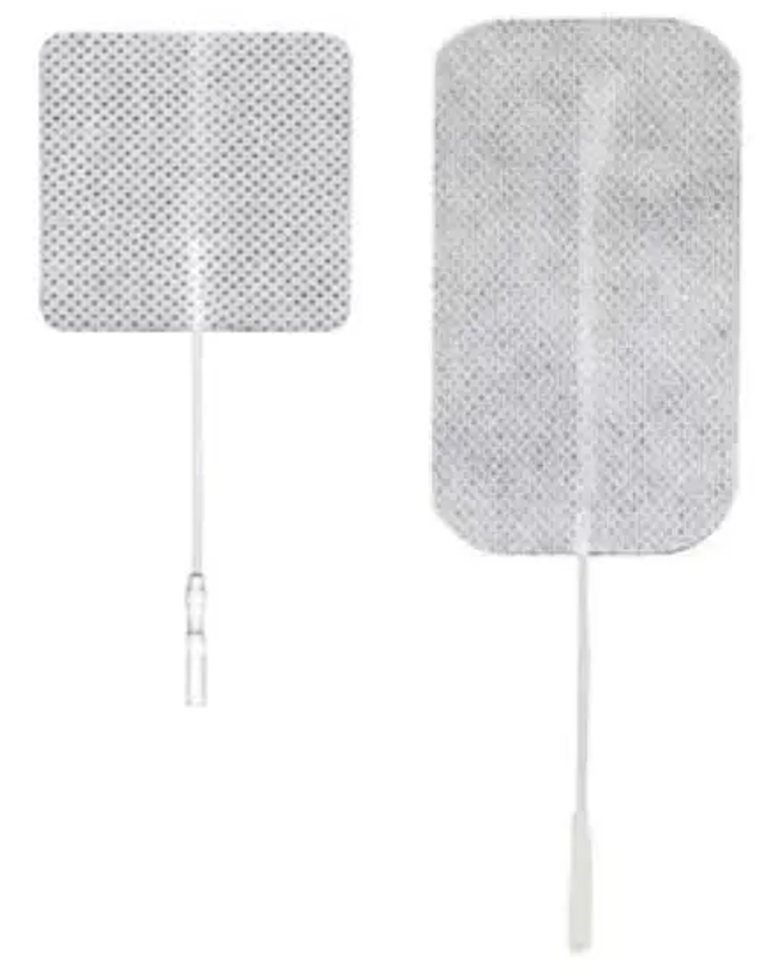
\includegraphics[width=\linewidth]{images/electrodes.png}
    \caption{FES electrodes}
    \label{fig:electrodes}
\end{wrapfigure}

Every stimulated muscle thereby required two electrodes, one active electrode and one reference electrode. Both 5x5cm and 5x9cm electrodes were used for this project (figure \ref{fig:electrodes}), depending on the muscle size. The connection was realized using cables with banana connectors, visible in figure \ref{fig:stimwave}. The chosen electrodes are equiped with adhesive gel creating a relatively stable electrode-tissue interface. 

\subsubsection{Electrode placement}
The placement of electrodes is an critical factor for achieving effective stimulation. It determines the quality of muscle activation the specificity and the comfort for the user. However, the optimal placements for each muscle is highly subject-dependent which makes the process of finding the placements challenging and time consuming.

To establish some form of systematic approach the optimal placements were first found in myself. This involved iteratively adjusting the placement of both the active and reference electrode positions, observing the muscle responses at different amplitudes and the discomfort level until a functional movement was achieved under the pain threshold (maximum tolerable intensity). Physiologically, optimal electrode placement aligns with the motor points of the targeted muscles \todo{source}. Motor points are regions where the motor nerve enters the muscle, resulting in the lowest threshold for activation thus minimizing discomfort and fatigue \todo{source}. To find the optimal placements for each muscle several sources were consulted with the most used source being an atlas of the muscle motor points by A. Botter \cite{botter_atlas_2011}. 

\begin{figure}
    \centering
    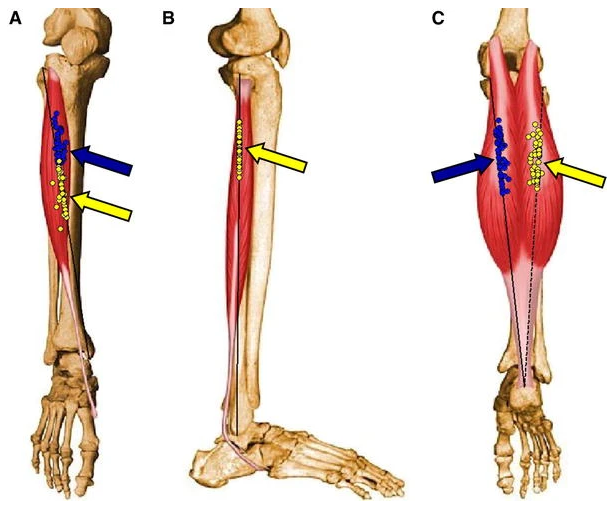
\includegraphics[width=0.6\linewidth]{images/screenshotmotorpoint.png}
    \caption{Example of motor points according to \cite{botter_atlas_2011} for: \textbf{a.} tibialis anterior; \textbf{b.}peroneous longus; \textbf{c.} medial (\textit{blue circles}) and lateral (\textit{yellow circles}) gastrocnemii. }
    \label{fig:motor-points}
\end{figure}

To document the process and provide a reference for future users a series of videos was creates, where each video captures the intended functional movement elicited by optimal stimulation of a muscle. This offers a clear visual benchmark which could then be used when finding the correct placements for new users, thereby maintaining consistency and ensuring that the functional movements are sufficient before moving on to the full gait cycle functional electrical stimulation.

\subsection{Open Loop Stimulation Sequence}
\lhead{Implementation - Open Loop Stimulation Sequence}
The open loop stimulation sequence specifies which muscles should be stimulated, the duration oftheir activation adn the delays between activations. The sequence aims to replicate a single step (gait cycle) for one leg using FES. The final goal is to produce a step that feels and looks natural and is comfortable for the subject while being general enough to work for a variety of subjects.

\subsubsection{Testing the Existing Sequence}
Initially, it was beleived that a working open loop sequence had already been established by a previous student. However upon testing the sequence on two different subject it became clear that the sequence ineffective and did not produce a step. The muscle activation was observed to feel unnatural and uncomfortable and ultimatley failed to pelicate a smooth coordinated movement. It therefore became necessary to dermine whether these issues stemned from errors in the implementation or from issues with the sequence itself.

\todo{figures}

This initial sequence was based on electromyography (EMG) measurements of muscle activation during gait in two healthy subject. Therefore to evalueate the accuracy of the sequence the EMG measurements from the two subjects were compaired against a comprehensice, open-source dataset of EMG activity during gait \cite{camargo_comprehensive_2021}. The discrepancies between the two became immediately apparent. In gait phases where the dataset indicated that certain muscles-such as the vastus medialis, hamstrings,and gluteus maximus-should be largely inactive the EMG measurement from the two subjects showed significant activation. There are several likely causes for these inaccuracies uncluding noise, motion artifacts or the EMG sensors picking up activity from muscles. Since the stimulation sequence was based directly on this flawed data several muscles were being stimulated during periods where they should be entierly inactive. This is what lead to the failure of the sequence in reproducing a natural and functional gait cycle. Having confirmed that the issue lay in the sequence itself, rather than its implementation, the focus was shifted to designing an entirely new stimulation sequence.

\subsubsection{Finding a new sequence}

\textit{Graphical User Interface}

To facilitate the testing and tuning of new stimulation sequences a new graphical user interface (GUI) tab (figure \ref{fig:sequenceGUI})was created. This interface allowed real-time adjustments not only to the durations and delayes but also the sequence of the muscles. This is done by relating each muscle to a specific channel. This significantly accelerated the iterative process of testing and optimizing sequences. 

\begin{figure} [h]
    \centering
    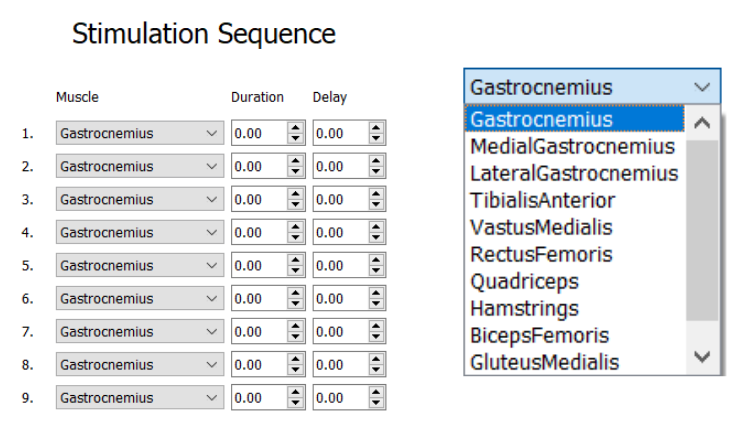
\includegraphics[width=0.8\linewidth]{images/sequenceGUI.png}
    \caption{Graphical user interface for testing new sequences.}
    \label{fig:sequenceGUI}
\end{figure}

\textit{Methodology}

In order to design a new sequence that would be robust literature insights from the literature relating to FES for gait and a seminal text on gait physiology were used. To ensure that the sequence aligned with natural muscle activation patterns, the seminal text \textit{Gait Anlysis: Normal and Pathological function} \cite{perry_gait_2024} was consulted. This book provides comprehensive descriptions of muscle activity throughout the gait cycle with exact start and top percentages of the gait cycle for nearly all lower extremity muscles during gait. However the gait stimulation sequence could not be based only on this. It would be impossible to stimulate every muscle individually as they are activated naturally, there are simply too many muscles and FES does not have the necessary selectivity to accomplish that. Unlike voluntary contractions, which selectively and smoothly activate specific motor units, FES broadly stimulates motor nerves, often activating muscles indiscriminately. Therefore it was necessary to choose only a few muscles to stimulate and to determine this the existing literature relating to FES was examined.

\begin{figure} [h]
    \centering
    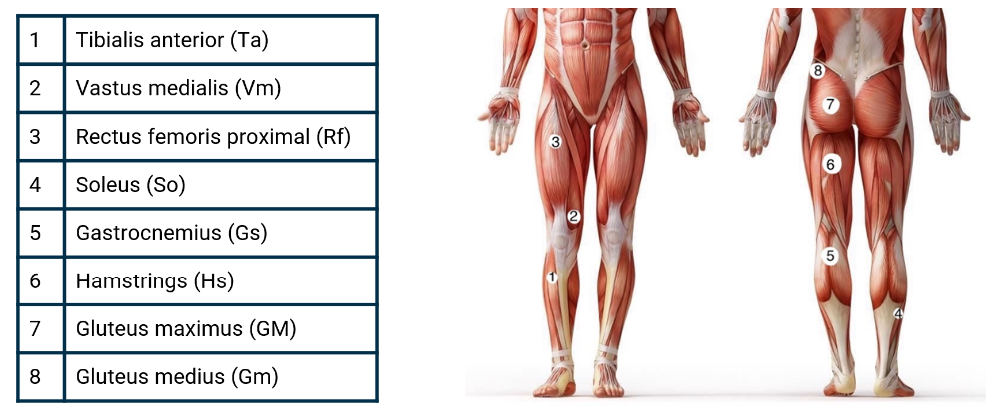
\includegraphics[width=0.85\linewidth]{images/common_muscles.png}
    \caption{Common muscles used for FES driven gait}
    \label{fig:commonMuscles}
\end{figure}

The literature ( \todo{sources}) revealed a large variety in the sequences used in FES gait studies. The timing end exact muscles varied greatly, however, the number of muscles was relatively consistent between four and eight and the tibialis anterior, gastrocnemis and biceps femoris (hamstring) appeared consistently in nearly all implementations. A list and visualization of the most common muscles is shown in figure \ref{fig:commonMuscles}. Several sequences inspired by physiological insights and the literature were tested. 
\newline \newline


\subsubsection{Six muscle Sequence}

First a sequence with six muscles: Tibialis Anterior, Gastrocnemi, Vastus Medialis, Hamstrings, Gastrocnemi and the Gluteus Maximus, was tested. This was the first sequence that produced a step. 

\subsubsection{Five muscle sequence}
The next sequence tested did not include the gluteus maximus, this was done to see whether the gluteus was necessary to stimulate. It had been pointed out by collegues experienced with running FES on patients that patients typically find the stimulation and placement process for the gluteus to be both challenging and uncomfortable. 

The hypothesis was that the gluteus Maximus may not be necessary to stimulate since several studies using FES to produce gait did not include the gluteus muscles ( \cite{aout_effects_2023} \todo{sources}). There are several reasons as to why the gluteus maximus, although important in natural gait, may not be necessary to stimulate. The first is muscle compensation. The gluteus is mostly involved in hip stabilization and hip extension. However the hamstring stimulation provides som hip extension that may be sufficient \todo{source}. The second is that the gluteus is primarily active during activities that require powerful hip extension such as climbing stairs or running \todo{source}. For flat ground however, especially at slower speeds the gluteus may play a smaller role. 

This new sequence also produced a step that did not seem of a lower quality than the sequence that included the gluteus. The stimulation was also noted to be more comfortable without the gluteus, therefore it was decided that the gluteus could be removed from the sequence.



\subsubsection{Four muscle sequence}
Next a sequence without the Rectus Femoris was tested, this was done due to several observations. Firstly, during experiments it was observed that stimulating only the Vastus Medialis led to a full knee extension leading to questions as to why the Rectus Femoris must be stimulated as well. The rectus femoris functions in both hip flexion and knee extension during natural gait, however upon FES stimulation it mostly produces an extension. So a hypothesis was formed that they knee extension needed may be achieved through stimulation of only the Vastus Medialis which focuses solely on knee extension without impacting hip movement. 

Secondly on experimentation done on myself it proved difficult to find a comfortable electrode placement for rectus femoris, and stimulating the rectus femoris proved to be the most uncomfortable muscle to stimulate. This was also corrobarated as a typical experience among patients by experienced collegues. 

Finally it was observed that there was a large discrepancy between when the Rectus Femoris was being stimulated in the literature compared to when it was active during natural gait according to the physiology. In fact in the literature it was largely being used for knee extension, while physiologically this muscle is mostly active during the initial-swing and mid-swing phases where it provides foot clearance and does not act as an extensor at all. 

\begin{figure} [h]
    \centering
    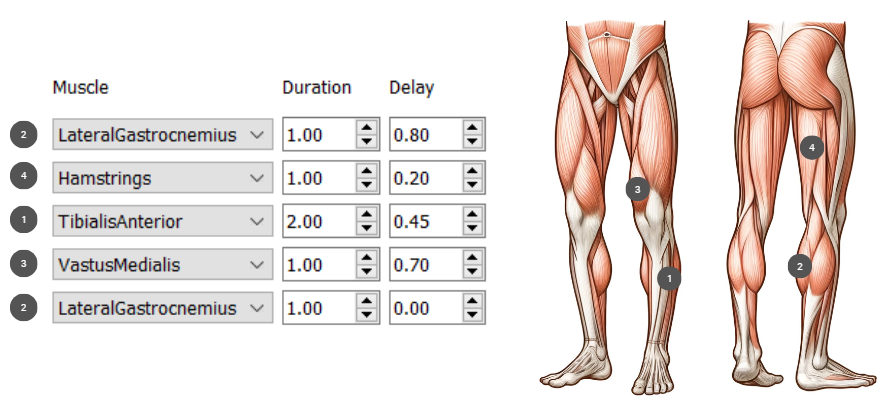
\includegraphics[width=0.99\linewidth]{images/final_seq_w_muscles.png}
    \caption{Final muscles and sequence}
    \label{fig:fianlsequence}
\end{figure}

When testing a new sequence without the rectus femoris there was no discernible difference between the steps produced when looking at videos of the respective sequences. The sequence also proved to be more comfortable leading to the conclusion that the Rectus Femoris may be removed from the sequence. This sequence visualized in figure \ref{fig:fianlsequence} ended up being the final sequence chosen, with results on multiple subjects available in the result section on the open loop stimulation sequence.



\lhead{Implementation - IMU implementation}
\subsection{IMU implementation}
\begin{wrapfigure}{r}{0.5\textwidth}
        \centering
    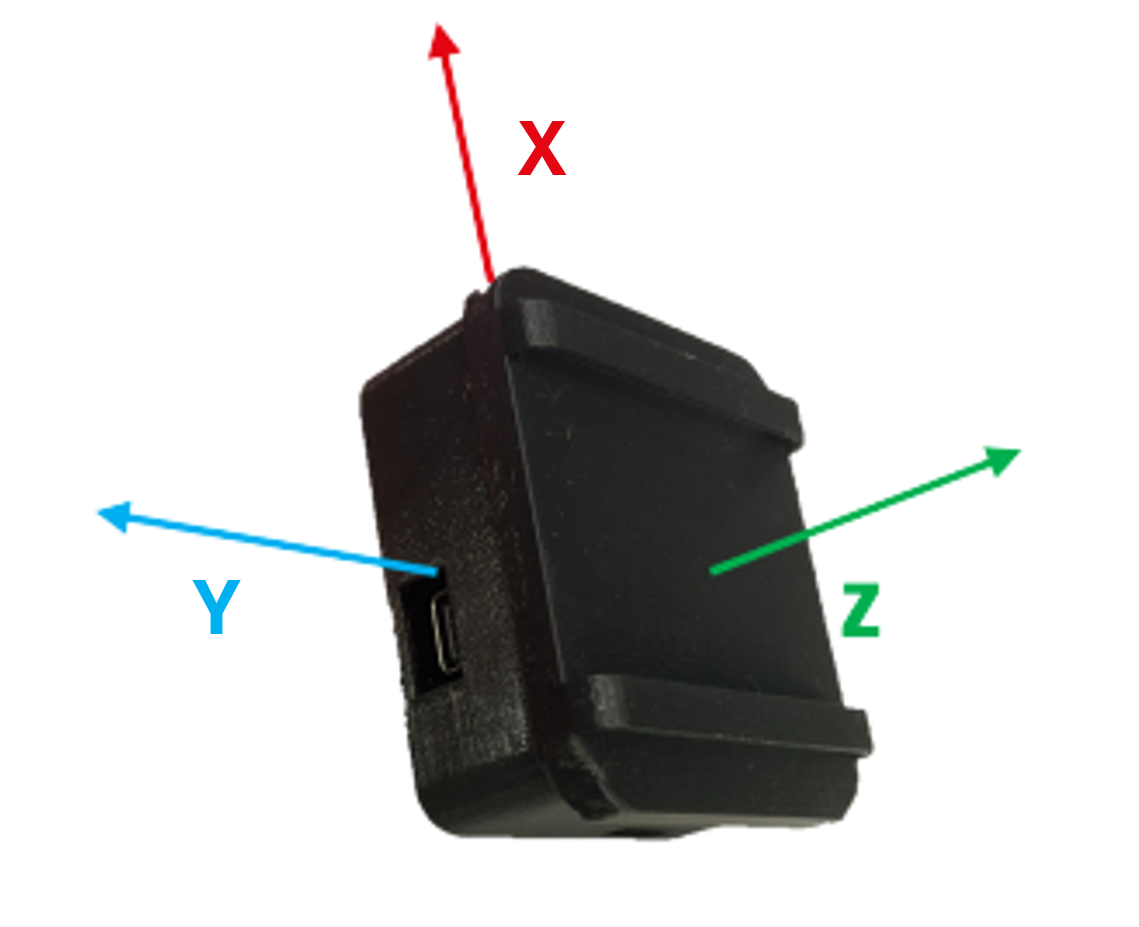
\includegraphics[width=\linewidth]{images/IMU_directions.png}
    \caption{New wireless IMU}
    \label{fig:imudirection}
\end{wrapfigure}
A part of the project involved replacing the old wired IMUs used by the previous student, with new wireless IMUs developed at the laboratory. These new IMUs enhance the portability and adaptability of the system, making them better suited for this application. They feature a high sampling frequency of 1kHz, and are capable of communicating using the Lab Streaming Layer (LSL) protocol. LSL is a real-time communication framework that allows data from multiple devices to be syncronized and recorded with low latency \todo{source}. The IMUs continuously transmit acceleration and angular velocity data via LSL, providing a high-resolution stream of motion information.

The transition to wireless IMUs required adapting the C++ code base to be able to receive the LSL-based data streams. Code from students working on gait phase detection in Python provided a starting point, as it already included functionality for connecting to the IMUs and accessing the data streams. The primary task was therefore to replicate and adapt this functionality in C++ in the refactored codebase. This involved setting up connections to the LSL streams emitted by the IMUs. Each device was configured as an independent source, transmitting real-time data. Modular code using threading was developed to ensure that the connection setup, data acquisition and processing could handle multiple IMUs simultaneously. The use of multithreading ensured that data from each IMU could be processed concurrently. 

\begin{figure} [h]
    \centering
    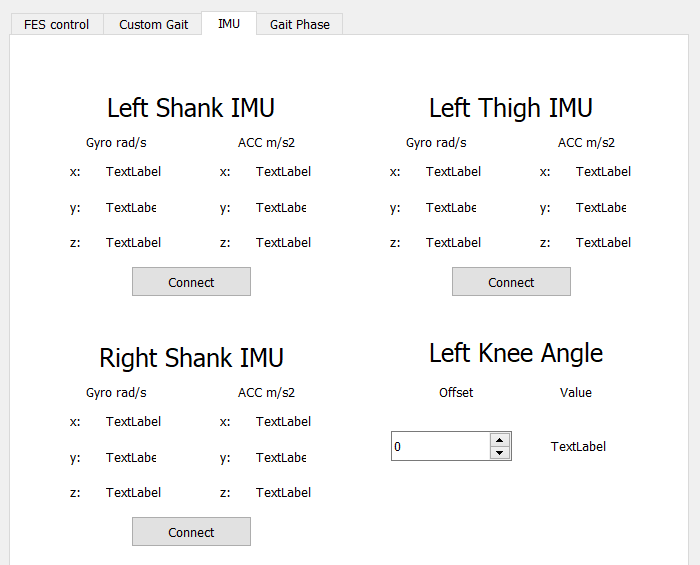
\includegraphics[width=0.7\linewidth]{images/imugui1.png}
    \caption{Graphical User Interface for visualizing IMU values}
    \label{fig:imugui}
\end{figure}

A new tab for the GUI was also created in order to visualize the data in real time. A screenshot of the GUI can be seen in figure \ref{fig:imugui}. There were four IMUs available at the laboratory designated A, B, C and D and in the code these IMUs are assigned as either left or right, shank or thigh IMUs. This mapping may easily be changed, which is useful when working with wireless IMUs that need regular charging. The connect button trigger creation of a new instance of the IMU class and a new thread on which the data is processed and then sendt back to be visualized in the "TextLabel" fields.

\subsection{Knee Angle Estimation}
The feedback for the closed-loop control system was designed to rely on the knee angle, it was therefore necesary to implement a robust method of extracting the knee angle from the IMU measurements. This was done by mounting one IMU on the shank and onther on the thigh. The angle between these two segments could then be calculated using the relative orientation of the IMUs. However, determining this angle requires an algorithm capable of providing accurate, low-latency orientation estimates. 


\subsubsection{Algorithm Selection}
Simple integration of gyroscope data is not viable since the integration process in inherently sensitive to small inaccuracies in the gyroscope output which accumulate over time, causing the orientation to deviate from the true value - a phenomenon known as drift. These inaccuracies are inevitable not only because of the noise affecting IMU but also since this is a highly dynamic system. Therefore sensor fusion algorithms had to be evaluated.

It has been demonstrated in many publications (e.g. \cite{peng_cheng_joint-angle_2010}, \cite{sabatini_estimating_2011} and the sources therein) that IMU data can be used to calculate hinge joint angles. Hinge joint angles can be calculated by integrating the difference of both angular rates around the corresponding coordinate axis and several techniques have been suggested to eliminate drift using accelerometers \cite{peng_cheng_joint-angle_2010}. As time for this project is limited it was a priority to find an algorithm that would not be very time consuming to implement. Towards this end a popular python library named \textit{Attitude and Heading Reference Systems (AHRS)} \cite{noauthor_ahrs_nodate} was consulted with the aim of using the python implementations as starting off point for the necessary C++ implementation. Here three selected methods are compared and contrasted for this particular application. Three methods were selected based on their applicability, robustness and ease of implementation. 



\subsubsection{Madgwick Filter}

The Madgwick filter is a gradient-descent-based orientation estimation algorithm. It provides a computationally efficient framework to estimate the orientation based on using gyroscope data for the prediction step and accelerometer data for the correction step. 

\textit{Theoretical Implementation}
The Madgwick filter would be implemented on the thigh and shank IMUs individually. The implementation outlined here is adapted from the original internal report by S. Madgwick  \cite{madgwick_ecient_nodate} and the documentation of the AHRS implementation \cite{noauthor_madgwick_nodate}. In the madgwick filter the orientation of the sensor frame relative to the earth frame is represented as a quaternion \( \mathbf{q_{\omega , t}} \):
\[
\mathbf{q_{\omega , t}} = 
\begin{bmatrix}
q_w & q_x & q_y & q_z
\end{bmatrix}^T
\]
where \( q_w \) is the scalar part, and \( q_x, q_y, q_z \) are the vector components.

\textit{Prediction step: Integration of Angular Velocity}

The orientation quaternion is predicted by numerically integrating integrating the quaternion derivative 
\(
\dot{\mathbf{q}}_t = \frac{1}{2} \mathbf{q}_{t-1} \otimes \boldsymbol{\omega}_t
\) as:
\[
\mathbf{q}_{\omega, t} = \mathbf{q}_{t-1} + \dot{\mathbf{q}}_{\omega, t} \Delta t
\]
\[
\mathbf{q}_{\omega, t} = \mathbf{q}_{t-1} + \frac{1}{2} \left( \mathbf{q}_{t-1} \otimes \mathbf{S}\boldsymbol{\omega}_t \right) \Delta t
\]
where \( \Delta t \) is the sampling period and 
\(
\mathbf{S}\boldsymbol{\omega} = 
\begin{bmatrix}
0 & \omega_x & \omega_y & \omega_z
\end{bmatrix}
\)
is the tri-axial angular rate, in rad/s, measured in the sensor frame and represented as a pure quaternion. For a more detailed explanation on orientation estimation based solely on angular rate and quaternion kinematics the reader is referred to \cite{sola_quaternion_2017}.

\textit{Correction step: Gradient Descent}
To correct for gyroscope drift, the Madgwick filter uses accelerometer data to align the predicted gravity vector with the measure gravity vector. The objective funciton minimizes the error between the two:
\[
f(\mathbf{q}) = \mathbf{q}^* \otimes \mathbf{g} \otimes \mathbf{q} - \mathbf{a}
\]

Where  \( \mathbf{q}^* \) is the conjugate of the predicted quaternion. The reference gravity vector in the Earth frame is \(\mathbf{g} = [0, 0, 0, 1].\) and the normalized accelerometer measurement is
    \(
    \mathbf{a} = [0, a_x, a_y, a_z].
    \)

The gradient of the objective function is computed as:
\[
\nabla f(\mathbf{q}) = \mathbf{J}^T f(\mathbf{q})
\]

where \( \mathbf{J} \) is the Jacobian matrix of the objective function.

The corrected quaternion is updated using a gradient descent step:
\[
\mathbf{q}_{k+1} = \mathbf{q}_k - \mu \frac{\nabla f(\mathbf{q})}{\|\nabla f(\mathbf{q})\|}
\]

where \( \mu \) is the step size (gain), which controls the convergence rate.


\textit{Application to Knee Angle Estimation}

 The algorithm is used to estimate the orientation of each IMU relative to the Earth frame, yielding quaternions \( \mathbf{q}_{\text{thigh}} \) and \( \mathbf{q}_{\text{shank}} \). The knee angle is then computed as the relative orientation between the two IMUs.
The relative orientation quaternion is calculated as:
\[
\mathbf{q}_{\text{relative}} = \mathbf{q}_{\text{shank}} \otimes \mathbf{q}_{\text{thigh}}^*,
\]
where \( \mathbf{q}_{\text{thigh}}^* \) is the conjugate of \( \mathbf{q}_{\text{thigh}} \).

The knee angle \( \theta \) is derived from the relative orientation quaternion:
\[
\theta = \arccos{\left( 2q_w^2 - 1 \right)},
\]
where \( q_w \) is the scalar component of \( \mathbf{q}_{\text{relative}} \).

\textit{Evaluation}

The main advantages of the Madgwick filter are that it is computationally efficient, especially designed for low cost, noisy IMUs, does not introduce potentially problematic delays, it's theoretically robust due to the correction step, the quaternion-based representation avoids singularities associated with euler angles. However there are some potential limitations. It might be sensitive to accelerometer noise such as during foot strikes. With this implementation there is also an implicit assumption that the local coordinate axes align exactly with the knee joint axis, additionally there is the assumptions that the IMUs themselves are algined. However all sensor fusion algorithm found during this project would also have required the same assumptions. Therefore because of the applicability of the algorithm, theoretical robustness and ease of implementation the Madgwick filter was selcted and adapted in order to estimate the knee angle.

\subsection{Phase detection}

The initial closed loop design involved the use of gait phase detection for use in determining which muscles should be stimulated. The plan was therefore to implement an on-line phase detection algorithm. This has been worked on during this same semester by another student at the lab who has been implementing a phase detection and subphase detection algorithm in python. The plan thas therefore to take the algorithm already developed and adapt it for C++ and Qt. This was thought to fit within the timeframe of the project only since the hope was that it would quite straight forward to simply translate the python algorithm and run it on a separate thread.

\subsubsection{The Algorithm}
\todo{write a description of the algorithm by francesco}

\subsubsection{Implementation}

Once this task was started on however it became clear that it would not be as simple as hoped to implement. The issue was that the python implementation used a host of SciPy \cite{noauthor_scipy_nodate} functions in order to implement the algorithm. Scipy is a  widely used library for scientific computing in Python, providing modules for among other things signal processing. Unfortunately, no equicalent comprehensive library exists for C++ thaty could directly replace SciPy's functionality. After an extensive search for alternatives, it became clear that replicating the necessary SciPy functions would be unavoidable.

To address this, a new class, "GaitPhaseDetector" \todo {make into code text}, was created to house the custom utility functions and the detction algorithm itself. It proved time consuming and challenging to ensure that the new functions matched the exact functionality of the SciPy functions. Having the new functions match exactly the SciPy functionality was hugely important since the entire gait phase and subphase algorithm had been built and tuned based on the usage of these functions. Many of the SciPy functions depended on nested calls to other SciPy utilities and the logic could be challenging to interperet. Despite these challenges, the class was developed and initial results were promising, indicating some degree of success in detecting the peaks needed to then detect the phases of gait. 

\todo{figure of peaks}

However, upon further testing, it became clear that the results were inconsistent and unreliable. A possible contributing factor here might be the potential discrepancies in the implementation of the SciPy functions. Despite thorough efforts to accurately replicate the functionality, subtle differences likely persisted which can have impacted the algorithm's performance. 

Another major challenge was the need to retune some of the algorithm parameters. The detection algorithm has been meticulously tuned throughout months of work to achieve a reliable and generalizable gait phase detector. The parameters include thresholds for metrics such as peak widths, which were defined as the number of data entries on either side of a peak. This posed  a significant challenge during adaptation since even when the C++ implementation exactly replecated the method in which data aquisition was managed in the Python implementation ( stream inlet in while loop) the frequency of incoming data differed. This discrepancy necessitates the retuning of all parameters that rely on counting the number of data points. This is a time consuming process. This issue as well as the issue of replicating 

While the adaptation of the Python-based gait phase detection algorithm to C++ initially appeared feasible within the project
s timeframe, the complexity of replicating SciPy's functionality and retuning the algorithm's parameters introduces significant challenges leading to the conclusion that implementing on-line gait phase detection would not be feasible within the time-frame of the project. However the initial implementation of the GaitPhaseDetector class is implemented with the architecture and stands ready to be more further developed and finished by later students.

\subsection{Closed-Loop}
A closed-loop control system was implemented in order to improve the quality of the stimulated step while also minimizing fatigue. This was achieved by dynamically adjusting the current amplitude by using a  PI controller dynamically adjust the current amplitude so that only the required current to induce the desired movement was applied. The final closed-loop design takes into account the lack of a viable phase detection algorithm, as discussed previously. Instead, the system relies solely on knee angle feedback and uses a time-dependent reference knee angle.

\subsubsection{Closed-Loop design}
\todo{closed loop figure}
A visualization of the closed loop control flow can be seen in figure \todo{put in figure reference}. The closed-loop takes in a knee angle reference that is fetched based on the current time and the gait cycle duration from the knee angle reference curve. Based on the the current time and gait cycle duration the current gait cycle percentage is extracted and used to determine which subphase of the gait the system should be in, based on this the muscles to stimulate are determined. The muscles that correlate to each subphase are based on the open-loop stimulation sequence, and can be seen in figure \todo{create figure for muscles}. Then for each muscle that should be stimulated a PI tuned for that specific muscle is run and there is a feedforward current that is summed with the PI current in order to get the current that will be sent to the StimWave board which then stimulates the muscles of the user. From the IMUs attached to the thigh and shank of the leg that should be stimulated the knee angle is then extracted and used as a feedback. A picture of the electrode and IMU placements on a single subject can be seen in figure \todo{ref}.

\todo{IMU and electrode placement picture}


\subsubsection{Knee Angle Reference Curve}
In order to use the error in knee angle as an input for the PI control it is important to have a good reference. Thankfully there is a lot of collected data on knee range of motion during gait. Knee range of motion has a specific curve during the gait cycle \todo{source}, a typical example can be seen in figure \todo{figure reference} 
\todo{knee angle curve figure}
\newline 

\textit{Simplified Curve}

Two different approaches to creating the reference curve were attempted. The first involved simply re-creating the general shape and amplitude of the typical knee angle curve by combination of two sinus curves tuned by-hand. The resulting curve modeled as the sum of two sinusoidal components, defined as:
\[
y(x) =
\begin{cases}
A_1 \sin\left(2 \pi f_1 x + \phi_1\right) + C_1, & 0 \leq x \leq 40 \\
A_2 \sin\left(2 \pi f_2 x + \phi_2\right) + C_2, & x > 40
\end{cases}
\]
where the parameters are defined as:

For the first bump:
\[
A_1 = 11, \quad f_1 = \frac{0.1}{4}, \quad \phi_1 = \frac{\pi}{2} + 2\pi f_1 \cdot 20, \quad C_1 = 15
\]

For the second bump:
\[
A_2 = 30, \quad f_2 = \frac{0.1}{6}, \quad \phi_2 = -\frac{\pi}{2} + 2\pi f_2 \cdot 80, \quad C_2 = 34
\]

A visualization of this curve can be seen in figure \todo{ref}. When comparing this however with the typical knee angle curve there are some major differences such as the height of the end of the second sinus curbe and height of the valley between the two curves. Because of these discrepancies another approach was attempted.
\todo{simple curve figure}
\newline

\textit{Fitted Curve}

The second approach was based on extracting the curve by fitting a fourier series to the measured knee angle data during gait. A fourier series fitting is .... . Readers that unfamiliar with fourier series fitting are referred to \todo{source}. The data used for the fitting is from the open source data set of gait analysis measurements by camargo et al. \cite{camargo_comprehensive_2021}. For that dataset several subjects were fitted with, among other things, a goniometer attached to the knee angle in order to get exact measurements of the knee angle during walking on a treadmill. 

\todo{Knee angle fitted curve figure}

For extracting the curve a single dataset at t a single speed (approximately 1 m/s) was used. Then a Fourier seris is used to approcimate the periodic knee angle data. The series is expressed mathematically as:
\begin{equation}
f(x) = a_0 + \sum_{i=1}^{n} \left( a_i \cos(2\pi i x) + b_i \sin(2\pi i x) \right)
\end{equation}

\begin{itemize}
    \item \(a_0\) is the constant offset (mean value of the function).
    \item \(a_i\) and \(b_i\) are the Fourier coefficients for the cosine and sine terms, respectively.
    \item \(n\) is the number of harmonics, which determines the complexity of the approximation.
\end{itemize}

In order to extract coefficient that best fit the data \texttt{curve\_fit}  function from \texttt{SciPy} is used. the number of harmonics (\textit{n}) is set to 3 in porder to balance accuracy and computational efficiency. This number provides enough flexibility to capture the primary general shape of the motion without overfitting to noise or adding unnecessary complexity. The  final curve is plotted alongside the original data in figre \todo{ref} which demonstartes how well the Fourier series captures the periodic behavior of the knee angle during gait. This improved resemblance to a physiological knee angle curve and since there is only a small change in computational complexity online with this more complicated equation led to the fitted curve being chosen as the curve used for the closed-loop implementation.
\todo{Knee angle fitted curve w data figure}.
\newline

\textit{Implementation}

In order to use the fitted curve as the reference for the PI controller, the knee angle corresponding to the current percentage of the gait cycle must be extracted in real time. This process begins by determining which percentage of the gait cycle the system is currently in. This is calculated using the current time and the gait cycle duration set by the user. The corresponding knee angle is then retrieved from the fitted curve. Which is then fed to the PI controller.

\subsubsection{Gait Cycle Duration}
As mentioned the reference knee angle degree value depends on the gait cycle duration and current time, therefore setting the correct gait cycle duration for each user is an important step. Gait cycle duration defines the time required for one complete stride, encompasssing the full sequence of movements from both legs. 

When running the FES experiments on a treadmill this gait cycle duration will vary from user to user and is therefore important to calculate before starting the stimulation. The primary input is the treamill speed (\(v\)) in (m/s). The second essential parameter is the subjects leg length (\(L\)), measured as teh distance from the greater trochanter to te floor in meters \todo{source}. Then the Froude number (\(Fr)\) which is a widely used descriptor in gait analysis is:
\begin{equation}
    Fr = \frac{v^2}{g \cdot L}
\end{equation}
Where g is gravitational acceleration. Once the Froude number is calculated the stride frequency (\(f_s\)) can be estimated using the following relationship \todo{source}:
\begin{equation}
    f_s = \sqrt{\frac{g \cdot Fr}{L}}
\end{equation}
From which the gait cycle duration is extracted and inserted into the program to ensure that the closed loop runs on a gait cycle duration that is comfortable for the user.


\subsubsection{PI controller}
To dynamically adjust the current amplitude based on the error between the desired and actual knee angle, a proportional-integral (PI) controller was implemented and tuned for each muscle independently. 
\newline

\textit{Controller choice}

The PI controller was chosen for its ability to address the system's specific needs.  Even though the reference angle changes over time a proportional-only controller may not adequately address persistent and steady-state errors as it only responds to the instantaneous error. Adding the integral term which accumulates error over time, effectively compensates for any consistent offset (e.g. under- or over-stimulation) that the proportional term cannot eliminate. 

\todo{Dicrete PI controller figure}

In a FES system, delays in muscle activation and mechnical response can cause the actual knee angle to lag behind the desired reference. By including an integral term the controller accounts for these delays indirectly: if the knee angle lags due to delayed muscle response, the accumulateed error promts the system to apply a sustained correction to minimize the offset over time.

The justification for not including a derivative term is that even though the derivative term would in theory enhance the responsiveness to rapid changes it would also implify the noise in the system. The IMU measurements and subsequent knee angle calculation is noisy and including a derivative term could quickly destabilize the control loop.
\newline 

\textit{Implemetation for FES}

The PI controller was implemented in the \texttt{LoopController} class based on the following discrete time equation:
\begin{equation}
I_{PI}(t) = 
\begin{cases} 
-K_p \cdot e(t) - K_i \cdot \frac{\Delta t}{2} \left(e(t) + e(t-\Delta t)\right), & \text{if extension phase} \\
K_p \cdot e(t) + K_i \cdot \frac{\Delta t}{2} \left(e(t) + e(t-\Delta t)\right), & \text{otherwise}
\end{cases}
\end{equation}

Where \( e(t-\Delta t) \) is the error at the previous time step. As is clear from the formula the integral term is calculated using trapezoidal integration. By averaging the error values at the start and end of the interval the trapezoidal approavh better captures the varying nature of the error compared to rectangular integration which assumes that the error remains constant during the interval \(\delta t\). It also reduces the likelihood of abrupt changes to the PI output since it accounts for error trends between time steps rather than using just the current error.

The PI controller also incorporates a phase-specific adaptation. This is because in knee extension increasing the stimulation of the extensor muscles decresases the knee angle, while increased stimulation of flexion muscles will increase the knee angle. To prevent counterproductive stimulation the controller therefor inverts its output during extension.


\subsubsection{Feedforward Current}
A feedforward current is implemented for each muscle individually to provide a baseline stimulation amplitude, ensuring sufficient activation to induce movement. It is set around the midpoint between the motor threshold and the maximum tolerable intesity found for each muscle during setup. 

Including a feedforward current is particularly beneficial in FES systems because it provides a consisten baseline for muscle activation reducing reliance on reactibe feedback adjustments and ensuring smotther, more predictable responses during the giat cycle. It also helps address delays in muscle activation and mechenical response by esnuring timely stimulation even before feedback corrections take effect. Additionally, the feedforward current reduces the workload on the feeback controller by offloading the need for large corrective actions requiring large gain values, allowing the controller to focus on fine-tuning adjustments.

Finally the feedforward current contributes to minimizing muscle fatigue by ensuring that the stimulation is applied more evenly over time. This reduces the need for large corrective currents, which could otherwise lead to over-stimulation and discomfort.


\subsubsection{FES stimulation}
The final calculated current is the sum of the feedforward current and the PI computed current saturated for safety reasons. The maximum possible current amplitude is the maximum tolerable intensity found during the setup and is set for each muscle individually. This saturated current is sent to the StimWave which then applies the stimulation with the set current amplitude, frequency and pulse width to the electrodes for each active muscle.


























 





































%=================================================================
%                           End Document
%=================================================================
\end{document}